\chapter{Numerical Solution of Flow Equations}
\label{chapter-three}

In this section, the discretization and method of solution of the governing
equations from \cref{chapter-two} is derived.  Traditionally, the reacting gas
path of FUN3D\cite{biedron2016fun3d} has employed an implicit, fully coupled
scheme in the flow solver.  In addition to providing details of this fully
coupled scheme, a decoupled scheme based on the Roe FDS scheme\cite{roe} is
derived to improve the computational efficiency of the flow solver and decrease
the relative memory required.  Details on the reconstruction scheme used in
FUN3D to extend the baseline finite-volume scheme to higher-order accuracy are
also provided in this section.

\section{Fully-Coupled Point Implicit Method}

The governing equations presented in \erefs{species-cons}{tot-energy-cons} can
be recast in vector form as
%------------------------------------------------------------------------------%
\begin{equation}
	\label{inv_flux_vec}
	\frac{\partial \mathbf{U}}{\partial t}
	+ \nabla\cdot \mathbf{F} = \mathbf{W}
\end{equation}
%------------------------------------------------------------------------------%
 or, in semi-discrete form,
%------------------------------------------------------------------------------%
\begin{equation}
	\label{inv_flux_fv}
	\frac{\partial \mathbf{U}}{\partial t}
	 + \frac{1}{V}\sum\limits_{f}(\mathbf{F}\cdot\mathbf{N})^f = \mathbf{W}
 \end{equation}
%------------------------------------------------------------------------------%
summing over all faces, $f$, in the domain, where V is the cell volume, 
$\mathbf{W}$ is the chemical source term vector, and $\mathbf{N}$ is the face
outward normal vector.  The vectors of conserved variables and fluxes are:
%------------------------------------------------------------------------------%
\begin{equation}
	\begin{matrix}
	\mathbf{U}=\begin{pmatrix}
   		\rho_1\\
		\vdots \\
		\rho_{ns} \\
		\rho u \\
		\rho v \\
		\rho w \\
		\rho E \\
	\end{pmatrix},      &
 	\mathbf{F} = \begin{pmatrix}
		\rho_1  \overline{U} \\
		\vdots \\
		\rho_{ns} \overline{U} \\
		\rho u \overline{U} + p n_x\\
		\rho v \overline{U} + p n_y\\
		\rho w \overline{U} + p n_z\\
		(\rho E + p) \overline{U} \\
	\end{pmatrix}
	\end{matrix}
  \label{fc-variables}
 \end{equation}
%------------------------------------------------------------------------------%
where $\overline{U}$ is the outward pointing normal velocity, $E$ is
the total energy of the mixture per unit mass as defined in
\eref{tot-energy-def}.  The flux and species chemical
source term at the next time level can be approximated as
%------------------------------------------------------------------------------%
\begin{equation}
	\begin{matrix}
		\mathbf{F}^{n+1} \approx \mathbf{F}^n+\frac{\partial \mathbf{F}}{\partial \mathbf{U}}\delta\mathbf{U}^n \\
		\\
		\mathbf{W}^{n+1} \approx \mathbf{W}^n+\frac{\partial \mathbf{W}}{\partial \mathbf{U}}\delta\mathbf{U}^n \\
	\end{matrix}
  \label{fc-fluxes-timelevel}
\end{equation}
%------------------------------------------------------------------------------%
where $\delta\mathbf{U}^n = \mathbf{U}^{n+1}- \mathbf{U}^{n}$.  Using an
implicit time integration, the implicit scheme becomes:
%------------------------------------------------------------------------------%
\begin{equation}
	\frac{\mathbf{\delta U}^n}{\Delta t}+\frac{1}{V}\sum\limits_{f}(\frac{\partial \mathbf{F}^f}{\partial \mathbf{U^L}}\delta\mathbf{U}^L
	+\frac{\partial \mathbf{F}^f}{\partial \mathbf{U^R}}\delta\mathbf{U}^R)^n \mathbf{N}^f
	- \frac{\partial \mathbf{W}}{\partial \mathbf{U}}\delta\mathbf{U}^n
	= -\frac{1}{V}\sum\limits_{f}(\mathbf{F}^f\cdot\mathbf{N}^f)^n + \mathbf{W}^n
\end {equation}
%------------------------------------------------------------------------------%
or, put more simply:
%------------------------------------------------------------------------------%
\begin{equation}
	A\delta\mathbf{U}^n = \mathbf{b}
\end{equation}
%------------------------------------------------------------------------------%
where $A$ is the Jacobian matrix of the fully coupled system, and $\mathbf{b}$
is the residual vector.  For a point implicit relaxation scheme, the Jacobian
matrix can be split into its diagonal and off-diagonal elements, with the latter
moved to the RHS:
%------------------------------------------------------------------------------%
\begin{equation}
\label{decomp-jac}
	A=O+D
\end{equation}
%------------------------------------------------------------------------------%
Each matrix element is a square $(ns+4)\times(ns+4)$ matrix.  This system can
be solved iteratively by using a multi-color matrix ordering to perform a series
of Gauss-Seidel sweeps. The computational work for the Gauss-Seidel scheme is
dominated by matrix-vector multiplications of elements of $O$ with
$\delta \mU$, which are $O((N_s + 4)^2)$ operations.  In the next
section, it is shown that decoupling the system reduces these matrix-vector
multiplications to $O(5^2 + N_s)$ operations.

\section{Decoupled Point Implicit Method}

If the species mass equations are replaced by a single mixture mass equation,
the mixture equations can be separated from the species mass
equations and the conserved variables become
%------------------------------------------------------------------------------%
\begin{equation}
	\mU' =
  \begin{pmatrix}
		\rho \\
		\rho u \\
		\rho v \\
		\rho w \\
		\rho E
	\end{pmatrix} \quad
	\Uhat =
  \begin{pmatrix}
		\rho_1 \\
		\vdots \\
		\rho_{ns}
  \end{pmatrix}
  \label{dc-variables}
\end{equation}
%------------------------------------------------------------------------------%
with corresponding flux vectors
%------------------------------------------------------------------------------%
\begin{equation}
 	\vF' = 
  \begin{pmatrix}
		\rho \overline{U} \\
		\rho u \overline{U} + p n_x\\
		\rho v \overline{U} + p n_y\\
		\rho w \overline{U} + p n_z\\
		(\rho E + p) \overline{U} \\
	\end{pmatrix} \quad
 	\Fhat = 
  \begin{pmatrix}
		\rho_1  \overline{U} \\
		\vdots \\
		\rho_{ns} \overline{U} \\
	\end{pmatrix}
  \label{dc-fluxes}
\end{equation}
%------------------------------------------------------------------------------%
Solving the flux vectors is performed in two sequential steps.  The mixture
fluxes, $\vF'$, are first solved as
%------------------------------------------------------------------------------%
\begin{equation}
  \frac{\partial \mathbf{{U}'}}{\partial t} +
  \frac{1}{V}\sum\limits_{f}(\mathbf{F}'\cdot\mathbf{N})^f = 0
\end{equation}
%------------------------------------------------------------------------------%
followed by the species fluxes, $\Fhat$, as
%------------------------------------------------------------------------------%
\begin{equation}
  \frac{\partial \mathbf{\hat{U}}}{\partial t} +
  \frac{1}{V}\sum\limits_{f}(\mathbf{\hat{F}}\cdot\mathbf{N})^f =
  \mathbf{\hat{W}}
\end{equation}
%------------------------------------------------------------------------------%
The same point-implicit relaxation that uses multi-color Gauss-Seidel sweeps is
used to update the conserved variables in $\mU '$, and all associated
auxiliary variables, such as temperature, pressure, speed of sound, etc. are
updated to be consistent with the new state of $\mU '$.  This update is done
holding the mass fraction state constant, and will always result in the
relaxation of a five-equation system.  Decoupling the variable sets in
\eref{dc-variables} does trade an implicit relationship between the mixture and
species equations for an explicit one; thus, this decoupling can have an impact
on the stability of the scheme, especially due to the non-linearity of the
chemical source term\cite{park}.
 
The solution of the species mass equations takes a different form.  Based on the
work of Candler et al.\cite{candler}, the decoupled variables can be rewritten
in terms of mass fraction, as follows:
%------------------------------------------------------------------------------%
\begin{equation} 
  \delta \Uhat^n 
  = \rho^{n+1} \Vhat^{n+1} - \rho^n\Vhat^n 
  = \rho^{n+1} \delta \Vhat^n + \Vhat^n \delta \rho^n
  \label{du-to-dv-mass-frac}
\end{equation}
%------------------------------------------------------------------------------%
where $\mathbf{\hat{V}}=(c_1,\hdots,c_{ns})^T$, and $c_s=\rho_s/\rho$ is the
mass fraction of species $s$.  While the derivation of the species mass
equations is different for the Roe FDS scheme from that of Steger-Warming
proposed by Candler et al.\cite{candler}, the final result takes a similar form: 
%------------------------------------------------------------------------------%
\begin{gather} 
  \hat{F}_{\rho_s} 
  = c_s F'_\rho+(c_s^L-\tilde{c}_s)\rho^L\lambda^+
  + (c_s^R-\tilde{c}_s)\rho^R\lambda^-
  \label{dc-flux}
\end{gather}
%------------------------------------------------------------------------------%
where $F_\rho'$ is the total mass flux computed previously using all
$\mathbf{U}'$ variables, $\tilde{}$ denotes a Roe-averaged quantity, and
$\lambda^{+/-}$ are functions of the Roe averaged eigenvalues.  Likewise,
linearizing the species mass fluxes with respect to the $\mathbf{\hat{V}}$
variables yields
%------------------------------------------------------------------------------%
\begin{align} 
  \Fhat^{n+1} &=
  \Fhat^n 
  + \pd{\Fhat}{\Vhat^L} \delta \Vhat^L 
  + \pd{\Fhat}{\Vhat^R} \delta \Vhat^R
  \label{flux-dc-taylor} \\
  \pd{\Fhat}{\Vhat^L} &= 
  \roe F_\rho+(1-\roe)\rho^L\lambda^+ - \roe \rho^R\lambda^- 
  \label{dfdvl} \\
  \pd{\Fhat}{\Vhat^R} &= 
  ( 1-\roe )F_\rho+(\roe -1)\rho^L\lambda^+ + \roe \rho^R\lambda^- 
  \label{dfdvr}
\end{align}
%------------------------------------------------------------------------------%
A full derivation of \erefs{dc-flux}{dfdvr}, along with the definition of
$\roe$, is included in \aref{decoupled-flux-derivation}. The chemical source
term is linearized in the same manner as the fully coupled scheme; however, the
updated $\mathbf{U}'$ variables are used to evaluate the Jacobian, and the chain
rule is applied to linearize $\mathbf{\hat{W}}$ with respect to the species mass
fractions:
%------------------------------------------------------------------------------%
\begin{equation} 
  \What^{n+1} = \What^n + 
  \pd{\What}{\mU} \bigg|_{\mU '} 
  \pd{\mU}{\Vhat}
  \label{source-term-linearization}
\end{equation}
%------------------------------------------------------------------------------%
For simplicity of notation, we define
%------------------------------------------------------------------------------%
\begin{equation} 
  C = \pd{\What}{\mU} \bigg|_{\mathbf{U}'} \pd{\mU}{\Vhat}
  \label{c-source-term}
\end{equation}
%------------------------------------------------------------------------------%
The decoupled system to be solved becomes:
%------------------------------------------------------------------------------%
\begin{equation} 
  \begin{split}
    \rho^{n+1} \frac{\delta \Vhat^n}{\Delta t} &+ \frac{1}{V} 
    \lsum{f}{}{ \left( \pd{\Fhat^f}{\Vhat^L} \cdot \Norm^f \delta \Vhat^L 
    + \pd{\Fhat^f}{\Vhat^R} \cdot \Norm^f \delta \Vhat^R \right)^{n,n+1}} 
    - C^{n,n+1} \delta \Vhat^n \\ 
    &= -\frac{1}{V}\lsum{f}{}{
      \left( \Fhat^{n,n+1} \cdot \Norm \right)^f } 
      + \mathbf{W}^{n, n+1} - \frac{1}{V} R_\rho \Vhat
  \end{split}
\end{equation}
%------------------------------------------------------------------------------%
where
%------------------------------------------------------------------------------%
\begin{equation}
  R_\rho =
  \lsum{f}{}{\lsum{s=1}{N_s}{(\hat{F}_{\rho_s}^{n,n+1}\cdot\mathbf{N})}} 
  \label{decoupled-no-scaling}
\end{equation}
%------------------------------------------------------------------------------%
is included to preserve the constraint that the mass fractions
sum to unity, i.e., $\sum\limits_{s}{c_s}=1$, $\sum\limits_{s}{\delta c_s}=0$

Candler et al.\cite{candler2013analysis} later found that the decoupled scheme,
using a modified Steger-Warming flux splitting, was less stable than the fully
coupled scheme when large reaction rates were present, particularly for
exothermic reaction.  This same instability was observed in numerical
experiments for \eref{decoupled-no-scaling}.  To mitigate this issue, Candler et
al. proposed an alternative decoupling of variable sets that was more stable,
particularly if endothermic reaction dominated the flow.  Instead of
implementing this alternative decoupled scheme, \eref{decoupled-no-scaling} is
modified with a scalar scaling factor, $\omega_r$, on the chemical source term
$\mw^{n,n+1}$
%------------------------------------------------------------------------------%
\begin{equation} 
  \begin{split}
    \rho^{n+1} \frac{\delta \Vhat^n}{\Delta t}
    &+\frac{1}{V}
    \lsum{f}{}{
     \left(
       \pd{\Fhat^f}{\Vhat^L} \cdot \Norm^f \delta \Vhat^L
       + \pd{\Fhat^f}{\Vhat^R} \cdot \Norm^f \delta \Vhat^R
      \right)^{n,n+1}}
     - C^{n,n+1} \delta \Vhat^n \\
    &= 
    -\frac{1}{V}\lsum{f}{}{
      \left( \Fhat^{n,n+1} \cdot \Norm \right)^f
    } + (\omega_r) (\mw^{n,n+1}) - R_\rho
  \end{split}
  \label{decoupled-with-scaling}
\end{equation}
%------------------------------------------------------------------------------%
Ramping this scaling factor from zero to one over the course of timestepping the
solution to steady-state preserves robustness of the decoupled scheme, and
numerical experiments show that it has minimal impact on the convergence rate.
Typically, the large reaction rates are only present during the transients early
on in the simulation, and damping the source term during this phase does not
affect the final result, provided the ramping is completed before the end of the
simulation.

\section{Predicted Cost and Memory Savings of the Decoupled Implicit Problem}
\label{sec:predicted-cost-mem-savings}

In decoupling the species equations, the most significant savings comes from the
source term linearization being purely node-based\cite{gnoffo-tp}.  Solving the
mean flow equations is conducted in the same manner as the fully coupled system.
All entries in the Jacobian $A_m$ are linearizations of the mixture equation
fluxes, which results in $5\times5$ matrices. All entries in the Jacobian $A_d$
are linearizations of the species mass fluxes, which results in $ns \times ns$
matrices.  Because there is no interdependence of species, except through the
chemical source term, all contributions due to linearizing the convective flux
are purely diagonal $N_s \times N_s$ matrices.  Via \eref{decomp-jac}, we
decompose $A_d$ into its diagonal and off-diagonal elements, resulting in the
following linear system:
%------------------------------------------------------------------------------%
\begin{equation}
  \label{dc_sys} 
  \begin{pmatrix} 
    \Box & & & & \\ & \ddots & & & \\ & & \Box \\ & & & \ddots & \\ & & & & \Box
  \end{pmatrix}
  \begin{pmatrix}
    \delta \mathbf{\hat{V}}_1 \\ \vdots \\ \delta \mathbf{\hat{V}}_i \\ 
    \vdots \\ \delta \mathbf{\hat{V}}_{nodes}
  \end{pmatrix}
  =
  \begin{pmatrix}
    \hat{b}_1 \\ \vdots \\ \hat{b}_i \\ \vdots \\ \hat{b}_{nodes} 
  \end{pmatrix}
  -
  \begin{pmatrix}
    (\sum_{j=1}^{N_{nb}}{[\diagdown] \delta\mathbf{\hat{V}}_{j}})_1 \\ \vdots \\
    (\sum_{j=1}^{N_{nb}}{[\diagdown] \delta\mathbf{\hat{V}}_{j}})_i \\ \vdots \\
    (\sum_{j=1}^{N_{nb}}{[\diagdown] \delta\mathbf{\hat{V}}_{j}})_{nodes}
  \end{pmatrix} 
\end{equation} 
%------------------------------------------------------------------------------%
where $\Box$ represents a dense $N_s \times N_s$ matrix, $[\diagdown]$ represents
a diagonal matrix, and $\delta \mathbf{\hat{V}}_j$  is the decoupled variable
update on the node $j$ that neighbors node $i$, where $N_{nb}$ is the number of
nodes neighboring node $i$.  Thus, the non-zero entries in the off-diagonal
matrix can be reduced from diagonal matrices to vectors.  This results in
significant savings in both computational cost and memory, as the only expensive
operation left in solving the implicit system is dealing with the diagonal
entries in the Jacobian.  An LU decomposition of an $N \times N$ matrix
requires $\sim N^3/3$ operations, whereas the the matrix vector
products of equivalent dimension requires $N^2$ operations and the vector inner
products cost.  Including the LU decomposition operations, the relative cost of
the linear solves in the decoupled scheme compared to the fully coupled scheme
is approximately
%------------------------------------------------------------------------------%
\begin{equation}
  \text{Relative Computational Cost} = 
  \frac{
    \frac{\left( N_s + 4 \right)^3}{3} N_{nodes} + \left( N_s + 4 \right)^2(S_{GS})(N_{nz})
  }{
    \frac{(N_s)^3 + (5)^3}{3} N_{nodes} + \left( N_s + 5^2\right)(S_{GS})(N_{nz})
  }
  \label{relative-lu-gs-cost}
\end{equation}
%------------------------------------------------------------------------------%
where $S_{GS}$ is the number of multi-color Gauss-Seidel sweeps, $N_{nodes}$ is
the number of nodes, and $N_{nz}$ is the number of non-zero off-diagonal entries
stored using compressed row storage\cite{George}.  Because $(S_{GS)(N_nz} >>
N_{nodes}$, the LU decomposition cost is negligible except when the number of
species is extremely large.  $N_{nb}(N_s)$ operations.  If the LU decomposition
costs are dropped from \eref{relative-lu-gs-cost}, the relative cost of the
linear solve becomes
%------------------------------------------------------------------------------%
\begin{equation}
  \text{Relative Computational Cost} = 
  \frac{
   \left( N_s + 4 \right)^2
  }{
    \left( N_s + 5^2\right)
  }
  \label{relative-no-lu-gs-cost}
\end{equation}
%------------------------------------------------------------------------------%
and can therefore expect nearly linear speedup in the linear solver cost with the
number of species when using the decoupled system over the fully coupled system.
It should be noted that cost predicted by operation count of an LU decomposition
does not usually manifest equivalently in computational cost.  Significant
compiler optimizations are possible if a storage scheme is adopted where memory
collocation of the diagonal block jacobians is maintained.  These optimizations
decrease the cost of the LU decomposition relative to the Gauss-Seidel sweeps
further, and thus the LU decomposition has never been seen as a dominant cost
for hypersonic simulations.

Using compressed row storage, the relative memory savings in the limit of a
large number of species for the Jacobian is given by
%------------------------------------------------------------------------------%
\begin{equation}
  \label{mem_req_eq}
  \begin{split} 
    Relative\ Memory\ Cost &=
    \frac{size(A_d)}{size(A)} \\ &= \lim_{N_s\to\infty}
    \frac{(N_s^2+5^2)(N_{nodes})+(N_s+5^2)(N_{nz})}{(N_s+4)^2(N_{nodes}+N_{nz})} \\
    &= \frac{N_{nodes}}{N_{nodes} + N_{nz}}
  \end{split}
\end{equation}
%------------------------------------------------------------------------------%
For a three-dimensional structured grid, each node has six neighbors,
i.e., $N_{nz} = 6N_{nodes}$; therefore, we can expect the Jacobian memory
required to decrease by a factor of seven using this decoupled scheme.
Interestingly, for a grid that is not purely hexahedra, $N_{nz} > 6N_{nodes}$;
thus, this decoupled scheme provides higher relative memory savings on
unstructured grids than structured grids when using compressed row storage.

\section{Higher Order Reconstruction}
\label{sec:2nd-order-reconstruction}

To achieve higher-order accuracy, the FUN3D solver uses an extension of the
unstructured MUSCL (U-MUSCL) reconstruction scheme developed by Burg et
al\cite{burg2005higher,burg2003verification}, which is itself an extension of
the Monotonic Upstream-centered Scheme for Conservation Laws (MUSCL) scheme
developed by Van Leer\cite{van1979towards}.  The implementation is a combination
of central differencing and the original U-MUSCL scheme
%------------------------------------------------------------------------------%
\begin{equation}
  \begin{aligned}
    q_L &= q_1 + (1-\kappa)\left[ \phi\left( \pd{q_1}{x}dx + \pd{q_1}{y}dy +
    \pd{q_1}{z}dz \right) \right] + \frac{\kappa}{2}\left( q_2 - q_1 \right) \\
    q_R &= q_2 + (1-\kappa)\left[ \phi\left( \pd{q_2}{x}dx + \pd{q_2}{y}dy +
    \pd{q_2}{z}dz \right) \right] + \frac{\kappa}{2}\left( q_1 - q_2 \right)
  \end{aligned}
  \label{u-muscl}
\end{equation}
%------------------------------------------------------------------------------%
where $\kappa = 0.5$ is usually used on unstructured grids with mixed elements.
\fref{fig:edge-recons} shows that $q_{L,R}$ are the primitive variables at the
left and right sides of the edge midpoint, where the flux is evaluated,
$q_{1,2}$ are the primitive variables at nodes 1 and 2.
%------------------------------------------------------------------------------%
\begin{figure}[h]
  \centering
  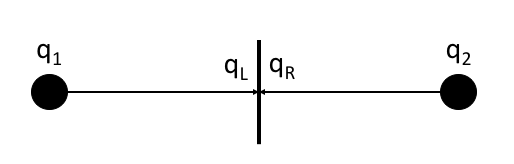
\includegraphics[width=0.5\textwidth]{figures/edge_reconstruction.png}
  \caption{Edge reconstruction.}
  \label{fig:edge-recons}
\end{figure}
%------------------------------------------------------------------------------%
The variable $\phi$ is the result of the scalar flux limiter function, that is
required to preserve monotonicity in the second order reconstruction near
discontinuities.  FUN3D supports a larger variety of flux limiters that fall
into two main categories: edge-based limiters, and stencil-based limiters.  The
edge based limiters are evaluated for two nodes at each edge.  Different values
of $\phi$ can exist at each node for edge-based limiter, and the results are not
``freezable'' at each node in FUN3D. Stencil-based limiters are evaluated at
each node, based on the gradients that are computed there.  For these limiters,
the value of $\phi$ is unique to each node and can be stored with the flow
solution as an additional variable.  The frozen state of the limiter is only
re-evaluated if the reconstruction forces a non-physical state at the dual
volume interface.

For this study, smooth Van Albada\cite{van1997comparative}, Van
Leer\cite{vatsa2009calibration}, and Minmod\cite{roe1986characteristic} flux
limiter functions are used.  Each of these limiters is augmented with a
heuristic pressure limiter by Park\cite{park2008anisotropic}. The choice of
these limiters impacts solution convergence and accuracy.  It is important to
note that the smooth Van Albada averaging function is given as
%------------------------------------------------------------------------------%
\begin{equation}
  \phi\left( a, b \right) =
  \frac{(b^2 + \varepsilon^2)a + (a^2 + \varepsilon^2)b}
  {a^2 + b^2 + 2\varepsilon^2}
  \label{van-albada-avg}
\end{equation}
%------------------------------------------------------------------------------%
where $a$ and $b$ are the left and right node gradients, and $\varepsilon$ is
the ``smoothing coefficient''.  This smoothing coefficient is used to tune the
flux limiter to a variety of the problems, and it is advised to be the
reciprocal of the mean aerodynamic chord (MAC) in grid units for
FUN3D\cite{biedron2016fun3d}.  The choice of $\varepsilon$ is critical to some
hypersonic applications involving chemistry, and will be discussed later.

